Numerical solutions to problems in quantum physics are important, given the limited availability of exact solutions. Many such models and methods exist when dealing with many-body systems, and have been shown to provide good estimates of physical behaviour \cite{}. Techniques such as Monte Carlo methods, exact diagonalisation, and DMRG are often used to solve a wide variety of many-body problems, but often fail to capture the full system dynamics of problems~\cite{}. To understand the behaviour of systems such as Bose--Einstein condensates, the use of these methods is incredibly limited. The increased complexity of the problem with increasing dimensionality of the system renders DMRG unusable. Exact diagonalisation requires a linear system to obtain realistic solutions, and also grows in complexity with increased dimensionality. Monte Carlo methods do not allow for real-time dynamics or yield much information about the underlying wavefunction. To obtain solutions to BEC problems I make use of a mean-field approach, outlined previously as the Gross--Pitaevskii equation \ref{sec:gpe}. Using the GPE and performing a numerical integration allows for almost all examinable dynamics that are valid in the mean-field theory. It can be noted though that the computational cost increases significantly with increased dimensions, and is already non-trivial for two-dimensions. I will lay the framework for the methods I have used to overcome this problem, and discuss the cutting edge numerical techniques involved.


\section{Time evolution}\label{sec:timeev}
One can write the wavefunction of a quantum system as a linear superposition of states as
\begin{equation}
    |\Psi \rangle = \displaystyle\sum\limits_{n} C_n |\Psi_n \rangle,
\end{equation}
where $| \Psi_n \rangle$ are a set of basis states for the system, with coefficients $C_n$. We next assume a unitary evolution operator of the form
\begin{equation}
   \mathscr{U}(t,t_0) = \exp\left(\frac{-i\mathcal{H}(t-t_0)}{\hbar}\right),
\end{equation}
where $\mathcal{H}$ is the Hamiltonian of the system. To time evolve our system from some time $t_0$ to a final time $t$ we apply the evolution operator to the wavefunction, giving
\begin{equation}
   \mathscr{U}(t,t_0)|\Psi \rangle = \displaystyle\sum\limits_{n} C_n \exp\left(\frac{-i{E_n}(t-t_0)}{\hbar}\right)|\Psi_n \rangle,
\end{equation}
where we have replaced the Hamiltonian operator with the energy eigenvalue of the $n$-th state. It follows from here that each state evolves at a different rate, proportional to its given eigenenergy; higher energy states will oscillate faster than those of lower energy states. As the groundstate of the system is always the most stable state, it is the one preferred by the system to set itself into.

Therefore, to create the initial state for the evolution scheme we consider the ground-state of the Hamiltonian. This can be achieved by evolving the system in imaginary time, causing all higher energy terms in an initial guess for the condensate wavefunction to decay to zero. This leaves the lowest energy state, which is the ground-state of the system. Taking the evolution operator, we apply a Wick rotation \cite{}, rotating the time component through $\pi/2$ into the imaginary plane, as $t \rightarrow -it$. Applying this new evolution operator to the wavefunction gives
\begin{equation}
       \mathscr{U^{'}}(t,t_0)|\Psi \rangle = \displaystyle\sum\limits_{n} C_n \exp\left(\frac{-{E_n}(t-t_0)}{\hbar}\right)|\Psi_n \rangle.
\end{equation}
This process removes the complex term in the operator, which now takes the form of sums of exponentially decaying states. When applied to the wavefunction all higher energy terms will decay at a rate faster than lower energy components. This process also causes a loss of probability density, and so the wavefunction must be renormalised after each application. Through repeated application of this operator, and a renormalisation afterwards, the simulated quantum system can converge to the ground-state solution. To begin, however, we must assume an initial guess for the wavefunction, which has some finite overlap with the lowest lying state. This method is a mathematical trick used to obtain a simulated ground-state, with a real-world system only tending to the ground-state in the presence of some form of dissipation.

As effective as this approach may be, the convergence to the lowest lying energy state becomes less effective as the computation approaches the expected value \cite{Vtx:Danaila_pra_2005}. Although many such methods exist to implement this, one that is well suited for this task is the Fourier split-operator method.

\section{Fourier split-operator method}\label{sec:numerics}
%For many of the works described previously, it is necessary to apply numerical techniques to obtain solutions. As the Gross--Pitaevskii equation, given in Eq. \eqref{eqn:gpe}, is used in the majority of the literature cited, we will consider it as the basis for the following discussion.
The Gross--Pitaevskii equation is a second order non-linear partial differential equation, and so very few exact solutions exist; the problem must often be tackled by a numerical approach. Though there are many ways to solve such a system numerically, with the Crank-Nicholson and Trotter-Suzuki algorithms being notable examples, the method I have chosen is the pseudospectral Fourier split-operator \cite{Num:Bauke_cpc_2011}.

If we consider a unitary evolution operator of the form
\begin{equation}\label{eqn:1}
\Psi(\mathbf{x},t+\tau) = \exp\left[ -\frac{i\hat{H}\tau}{\hbar}\right]\Psi(\mathbf{x},t),
\end{equation}
where $H$ is the Hamiltonian, composed of momentum, potential, non-linear interaction, and rotation terms defined in Eq. \eqref{eqn:gpe}, we can solve for the wavefunction, and its resulting dynamics over a specified time-scale. However, due to error propagation resulting from numerical integration, it is instructive to employ methods that allow for the highest precision while providing results in useful timescales. To allow for this, care must be taken during the implementation of such integration methods.  If we take the Hamiltonian, $\hat{H}$, in terms of its components as a combination of position and momentum space functions we obtain
\begin{equation}\label{eqn:2}
\hat{H} = \hat{H}_{\textbf{r}} + \hat{H}_{\textbf{k}} + \hat{H}_{\textbf{L}},
\end{equation}
where we first neglect the angular momentum operator, $\hat{H}_{\textbf{L}}$, and consider only the two other non-commuting parts $\hat{H}_{\textbf{r}}$, containing the position operator, and $\hat{H}_{\textbf{k}}$, containing the momentum operator. The Zassenhaus product of the Baker-Campbell-Hausdorf formula \cite{some citation} gives the relation for non-commuting operators as
\begin{equation}
    \exp\left( t(A+B) \right) = \exp\left(tA\right)\exp\left(tB\right)\exp\left(-\frac{t^2}{2}[A,B]\right)\cdots
\end{equation}
with $\cdots$ representing higher order commutators. This is directly mappable to the above Hamiltonian for time evolution. Given the non-commutativity of $\hat{H}_{\textbf{r}}$ and $\hat{H}_{\textbf{k}}$, the above expression cannot be evaluated exactly, and so it is common to Taylor expand and truncate the expression. The resulting error can be determined as
\begin{subequations}\label{eqn:error_calc}
\begin{align}
    \text{err} = \left\| \exp\left(-\frac{i\hat{H}_{\textbf{k}}\tau}{\hbar}\right)\exp\left(-\frac{i\hat{H}_{\textbf{r}}\tau}{\hbar}\right) - \exp\left(-\frac{i(\hat{H}_{\textbf{k}} + \hat{H}_{\textbf{r}})\tau}{\hbar}\right) \right\| \\
    = {\Biggl\|}  \left(1 + \left(\frac{-i\hat{H}_{\textbf{k}}}{\hbar}\right)\tau + \left(\frac{-i\hat{H}_{\textbf{k}}}{\hbar}\right)^2\frac{\tau^2}{2}  \right)\left(1 + \left(\frac{-i\hat{H}_{\textbf{r}}}{\hbar}\right)\tau + \left(\frac{-i\hat{H}_{\textbf{r}}}{\hbar}\right)^2\frac{\tau^2}{2}  \right) &-\\ \left(1 + \left(\frac{-i(\hat{H}_{\textbf{r}} + \hat{H}_{\textbf{r}})}{\hbar}\right)\tau + \left(\frac{-i(\hat{H}_{\textbf{r}} + \hat{H}_{\textbf{r}})}{\hbar}\right)^2\frac{\tau^2}{2}  \right)  + \mathcal{O}(\tau^3) {\Biggr\|}
\end{align}
\end{subequations}
which, upon simplification reduces to
\begin{equation}
\text{err} = \left\| \frac{\tau^2[{\hat{H}_{\textbf{r}}},{\hat{H}_{\textbf{k}}}]}{2\hbar^2} + \mathcal{O}(\tau^3)\right\| = \mathcal{O}(\tau^2).
\end{equation}

The error can be further reduced through the use of 2nd order Strang-splitting~\cite{strang-splitting}, reducing the error in the numerical integration scheme to $\mathcal{O}(\tau^3)$, with the resulting operator implementation given as

\begin{equation}\label{eqn:3}
\exp\left[ -\frac{ i\left(\hat{H}_{\textbf{r}} + \hat{H}_{\textbf{k}}\right)\tau}{\hbar} \right] = \exp\left[- \frac{i\hat{H}_{\textbf{r}}\tau}{2\hbar} \right]\exp\left[-\frac{i\hat{H}_{\textbf{k}}\tau}{\hbar}\right]\exp\left[ -\frac{i\hat{H}_{\textbf{r}}\tau}{2\hbar}\right] + \mathcal{O}\left(\tau^3\right).
\end{equation}
In the case of a nonlinear system, such as for solving the GPE, the above scheme attains a second-order error, resulting from the combination of the potential and nonlinear terms, with the respective mapping as \cite{BEC:Javanainen_jphysa_2006}
\begin{equation}
\hat{H}_{\textbf{r}} = V(\mathbf{r}) + g\vert\Psi(\mathbf{r},t)\vert^2\; \hspace{5em} \hat{H}_{\textbf{k}} = \frac{-\hbar^2}{2m}\nabla^2.
\end{equation}
%\hat{H}_{\textbf{L}} = \Omega L,
Following Bauke \textit{et al}. \cite{Num:Bauke_cpc_2011}, we can numerically solve this differential equation as
\begin{equation}
\Psi\left(\textbf{r},t+\tau\right) = \left[\hat{U}_{\mathbf{r}}\left(t+\frac{\tau}{2}\right) \mathscr{F}^{-1} \left[ \hat{U}_{\mathbf{k}}(t+\tau) \mathscr{F} \left[ \hat{U}_{\mathbf{r}}\left(t+\frac{\tau}{2}\right) \Psi\left(\mathbf{r},t\right) \right] \right] \right]  \\ + \mathcal{O}\left(\tau^2\right),
\end{equation}
where $\hat{U}_{r}(t)=e^{-i\hat{H}_{r}t/\hbar}$ is the time evolution operator in real space, $\hat{U}_{k}(t)=e^{-i\hat{H}_{p}t/\hbar}$ in momentum space,  $\mathscr{F}$ and $\mathscr{F}^{-1}$ are the forward and inverse Fourier transform respectively. Fig.~\ref{fig:num_splitop} outlines a schematic representation of the method during a single pass of the algorithm.

\begin{figure}
    \centering
    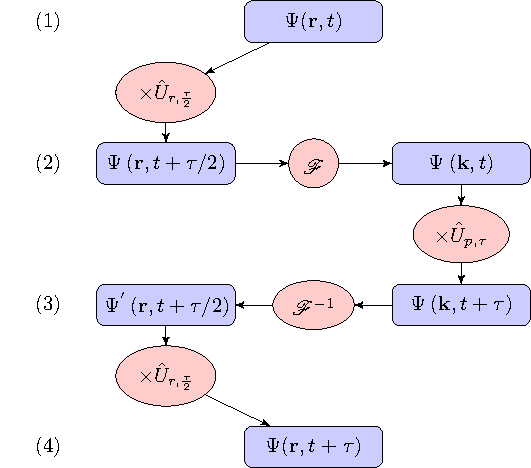
\includegraphics[]{./ch3_numerics/splitop}
    \caption{A single pass through the Fourier split-operator method.}
    \label{fig:num_splitop}
\end{figure}

The underlying theory of the Fourier split-operator method for the Gross--Pitaevskii equation is given by Javanainen \textit{et al}. \cite{BEC:Javanainen_jphysa_2006}, showing how the choice of non-linearity and operator splitting affects the outcome of the method. By taking the initial step as evolution in momentum space, the choice of the most current wavefunction attains an error of third-order for the algorithm. However, given the need for an additional two Fourier transform steps this is rather costly in compute time. For an initial step in position space, the nonlinear term is best calculated using a linear combination of all available wavefunctions through the algorithm $\Psi = c_0\Psi_0 + c_1\Psi_1 + c_2\Psi_2$, where the subscripts denote the wavefunction at each stage of the evolution in position space. This gives third order accuracy for the parameters $c_2=\pm 1, c_1=-c_0$. However, for simplicity and resource limitations I choose to work with the $\mathcal{O}\left(\tau^2\right)$ accurate scheme, which was sufficient for the works herein.

An implementation of this method is a straight-forward process using MATLAB, and has been performed for the purpose of this study. However, due to the computational overhead required to time-evolve such a system, the procedure takes a long time to simulate at the required degree of precision in anything higher than one-dimension. Therefore, it is necessary to further develop the methods used, and to improve the implementation of this algorithm to leverage the recent advances in computational acceleration.

\subsection{Resolution considerations}
As the Fourier split-operator method requires special consideration of resolution in both position and momentum space, care must be taken while choosing numerical grids. The reciprocal relationship between position and momentum space is known as \begin{equation}
    k_{\text{max}} = \frac{2\pi}{x_{\text{min}}},
\end{equation}
which follows the uncertainty relation; better resolution in one space, yields worse in the other. To allow for a condensate to be simulated effectively in both spaces, it must fit within the grid on which it is defined, and resolve to half the size of the smallest structure. It is easy to estimate a radius for the position space wavefunction, following the Thomas-Fermi limit. It is also rather easy to know that for a non-rotating condensate the wavefunction should occupy the lowest lying mode ($\mathbf{k}=0$), and those close to it, assuming a harmonic trap. Rotating the condensate, however, has the effect of expanding the wavefunction in position space due to centrifugal forces. Additionally, the momentum space wavefunction expands and occupies a larger space. With the addition of vortices to the system, there are now small scale structures to resolve. This leads to a difficult-to-simulate system; we have a simultaneously growing position space and momentum space wavefunction.

It is essential to have a large and finely sampled grid in order to resolve both position and momentum of the wavefunction. For my simulations a minimum grid-size on the order of $2^8$ for low rotation rates, to $2^{11}$ at high rotation rates in 2D for both $X$ and $Y$ dimensions to correctly resolve the system dynamics in both position and momentum space with vortices present. One such way of ensuring we can accurately resolve the system is to define a sufficient smallest length-scale on one such grid (such as position). With this, we can maintain a constant resolution in position space, whilst furthering momentum space resolution by increasing the number of samples of our grid. By ensuring the position grid remains defined with the same lowest increment, it is possible to increase resolution in the reciprocal space. Computationally, this is costly, but is quite effective when using compute accelerators (GPUs), which will be discussed later. %For the purpose of the work carried out herein, unless otherwise specified the simulations were resolved on a grid of $2^{10}\times 2^{10}$ elements, with spatial extent of the condensate $R\approx 700~\mu$m, and reciprocal space extent $K \approx 5\times10^{8}$ m$^{-1}$.
